\documentclass[11pt]{article}
\usepackage[T1]{fontenc}
\usepackage[utf8]{inputenc}
\usepackage{times}
\usepackage{amsmath}
\usepackage{framed}
\usepackage{graphicx}
\usepackage{hyperref}
\usepackage{fancyvrb}
\usepackage[english]{babel}
\title{{\bf LAB 1:\\Requirements Modeling}\\ Preparations and instructions}
\author{Björn Regnell}
\date{\today}
\begin{document}
\maketitle

\section{Introduction}

\subsection{Purpose} This document provides instructions on how to prepare for and run a computer lab session on requirements modeling. The lab session illustrates how computer-supported requirements modeling can help in requirements engineering, including elicitation, specification and validation. {\it The preparations in this document should be completed before the actual lab is run.}

\subsection{Background} Requirements engineering is a dynamic process where knowledge and perception of an imagined future system (of systems) is evolving over time. During this evolution we can capture the knowledge and creative ideas we elicit in various ways, depending on how we imagine the (later) usage of this information: we could create and use, for example, spread sheets, post-it notes, emails, wikis, video clips, mockups, sketches, diagrams, mathematical specifications, etc. 

If we want to keep track many different types of inter-related requirements and if we see a future benefit of more structure beyond just a flat list, we can use {\it requirements models} where requirements are expressed using relevant (meta-) {\bf entities}, {\bf attributes} and {\bf relations} that can capture what we want to model.   

The open source tool {\bf reqT} enables scalable requirements modeling, ranging from small models of a couple of features to large models containing elaborate structures of thousands of requirements. In this lab you will learn how to get started with reqT and reflect on how you could use reqT in your own project.

\clearpage\newpage
\section{Preparations}

Before the lab session, please complete all preparations below and bring requested items to the lab. In particular you need to make sure that you can access the text files you prepare below at your lab session computer.

\begin{enumerate}
\item {\bf Read reqT intro.} Read the section "Introduction to reqT" on this web page: \newline \url{http://reqt.org/documentation.html\#intro} 
\item {\bf Do the reqT "hello world".} Run the reqT hello world example on your computer, as explained here: \newline \url{http://reqt.org/documentation.html\#hello}
\item {\bf Draw a context diagram.} Draw a context diagram that  is relevant to your development project. Make the drawing on paper and bring to the lab. The context diagram should include entities outside of the system you are building that are communicating directly with the system under development. 
\item {\bf Create a context model.} Transform your context diagram into a reqT model, analogous to this  example: 
{\footnotesize\begin{verbatim}
Model(
  Product("hotelApp") interactsWith (
    User("receptionist"), 
    User("guest"), 
    System("telephony"), 
    System("accounting")))
\end{verbatim}}
Saved the model in a text file called \verb+context.scala+
\item {\bf Create a list of features.} Make a list of at least 5 features relevant to your project, divided into 2 sections, analogous to the example below. Use the exact formatting and indentation according to the example with hash tag before the name of each group and an asterisk before the name of each feature: 
{\footnotesize\begin{verbatim}
# receptionFeatures
  * groupCheckIn
    Check in many guests arriving in bulk.
# adminFeatures
  * roomForecast
    Calculate room allocation prediction.
  * exportAccounting
    Export accounting data to external system.
\end{verbatim}}
Saved the list of features in a text file called \verb+feat.txt+  
\end{enumerate}
\clearpage\newpage

\section{Lab instructions}

\subsection{Start reqT}
Download the reqT.jar file from \url{http://reqT.org} and start reqT in a terminal window using this command: \verb+java -jar reqT.jar+ as shown in Figure~\ref{fig:console}.

\begin{figure}[h]
    \centering
    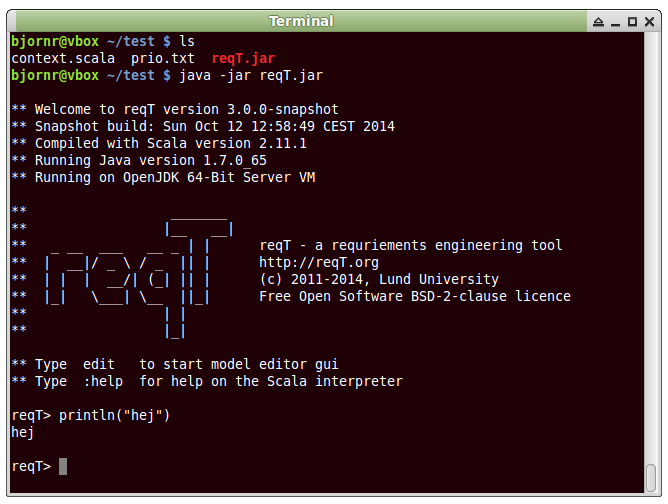
\includegraphics[width=0.8\textwidth]{console.png}
    \caption{The reqT console output after starting reqT in a terminal window.}
    \label{fig:console}
\end{figure}

\subsection{Create and update models using the reqT console}
Type in the following lines in the reqT console after the \verb+reqT>+ prompt. Press enter after each line. The \verb?+? operator is used to add elements to a model, and the  \verb?++? operator is used to append one model to another.

{\small\begin{verbatim}
reqT> val m1 = Model(Req("a") has Spec("sss"))

reqT> val m2 = m1 + (Req("b") has Prio(2))

reqT> val m3 = Model(Stakeholder("x") requires Req("a"))

reqT> ((m3 + Stakeholder("y")) ++ m2).size
\end{verbatim}}

\begin{framed}\noindent
Q1: What is the integer value result of the last evaluation? 
\newline 
\verb?((m3 + Stakeholder("y")) ++ m2).size?
\newline
\newline \underline{\hspace{11.9cm}}
\end{framed}

Continue to type in the following lines in the reqT console after the \verb+reqT>+ prompt. Press enter after each line. The \verb+for+ keyword is used to make a for-loop. The \verb+yield+ keyword is used in a for-comprehension to construct a sequence of values.  The \verb+val+ keyword is used to declare a name that refers to an immutable value (a constant) and the \verb+var+ keyword is used to declare a name that refers to a mutable value (a variable). The \verb?-? operator is used to remove elements from a model. With the \verb+transform+ method you can make transformations of specific elements in a model. 


{\footnotesize\begin{verbatim}
reqT> var m4 = (for (i <- 1 to 10) yield Req("r"+i)).toModel

reqT> (1 to 10).map(i => Req("r"+i)).toModel //alternative to above

reqT> m4 = Model(Stakeholder("x") requires m4)

reqT> m4 = m4 - Req("r7")

reqT> m4 -=  Req("r3")

reqT> m4.pp   //pretty-print m4

reqT> m4 = m4.transform{case Req(id) => Feature(id) has Status(ELICITED)}

\end{verbatim}}

\begin{framed}\noindent
Q2: What is the size of the m4 model after the above transform? 
\newline
\verb+m4.size+
\newline
\newline \underline{\hspace{11.9cm}}
\end{framed}

\subsection{Investigate the reqT metamodel}

A reqT model can be viewed as a vector of elements. Elements can be entities, attributes and relations. An entity has an id of type String. An attribute holds a value that can be of different types. A relation connects and entity via a link of a certain RelationType to a submodel that, in turn, can contain elements. A part of the reqT metamodel is shown in Figure~\ref{fig:metamodel}. 

\begin{figure}[h]
    \centering
    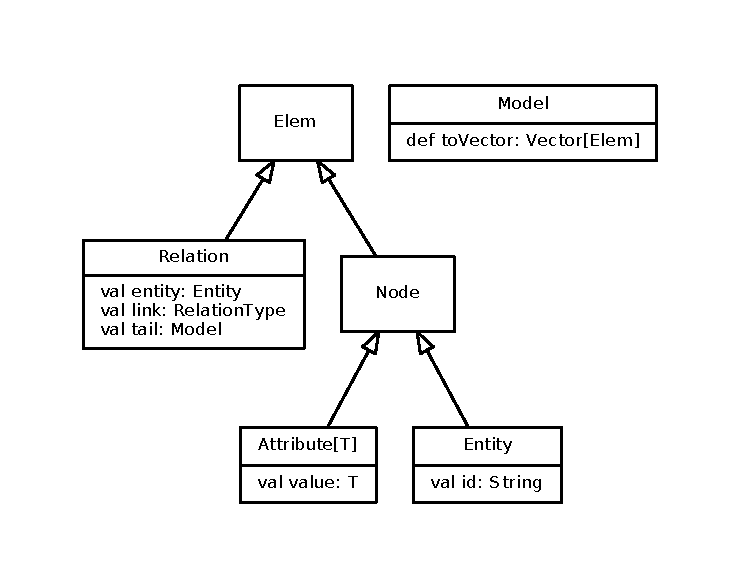
\includegraphics[width=\textwidth]{metamodel-simple.pdf}
    \caption{Some classes in the reqT metamodel.}
    \label{fig:metamodel}
\end{figure}

Investigate what different entity types, attribute types and relation types that the reqT metamodel contains, using the evaluations in the reqT console below. The collect method collects selected parts of a model into a vector. In the last evaluation below we collect the integer 1 for each occurrence of a Meta entity and sum all ones.

{\footnotesize\begin{verbatim}
reqT> reqT.metamodel.  // Press <TAB> after the dot

reqT> reqT.metamodel.ent // Press <TAB> after the t

reqT> reqT.metamodel.entityTypes

reqT> reqT.metamodel.entityTypes.size

reqT> reqT.meta.model.pp

reqT> reqT.meta.model.collect{case Meta(_) => 1}.sum
\end{verbatim}}

\begin{framed}\noindent
Q: How many different entity types, attribute types and relation types are there respectively in the reqT metamodel? 
\newline
\newline \underline{\hspace{11.9cm}}
\newline\newline
Q: How many \verb+Meta+ entity concepts are there in the reqT metamodel? 
\newline
\newline \underline{\hspace{11.9cm}}
\end{framed}

The meta model elements can be used in many different ways and there are no special restrictions on how to combine the elements, except for these three basic rules:
\begin{enumerate}
\item A model or submodel can only contain one attribute of a specific type at its top level. However, the same type of attribute can in different submodels. Try this in the reqT console:
{\footnotesize\begin{verbatim}
reqT> Model(Spec("a"), Spec("b"))
res1: reqT.Model = Model(Spec("b"))

reqT> Model(Req("x") has (Spec("a"), Spec("b")))
res2: Model(Req("x") has Spec("b"))

reqT> Model(Req("x") has Spec("a"), Req("y") has Spec("b"))
res3: Model(Req("x") has Spec("a"), Req("y") has Spec("b"))
\end{verbatim}}
\item A model or a submodel can only contain one entity with a certain id and a certain relation at its top level. If you add an entity with the same id and the same relation on the top level of a model or submodel, it will merge the elements of each submodel, and if the above rule applies attributes will be overwritten if of the same type. Try this in the reqT console:
{\footnotesize\begin{verbatim}
reqT> val m6 = Model(Req("x") has (Req("s1"), Spec("a"))) 

reqT> m6 + (Req("x") has (Req("s2"),Spec("b")))
res4: Model(Req("x") has (Req("s1"), Req("s2"), Spec("b")))
\end{verbatim}}

\item The has-relation is special, as an entity with no relation is equivalent to an entity with a has-relation to an empty submodel. Try this in the reqT console:
{\footnotesize\begin{verbatim}
reqT> Model(Req("x") has ())
res5: reqT.Model = Model(Req("x"))

reqT> Model(Req("x") has Spec("x")) - Spec("x")
res6: reqT.Model = Model(Req("x"))
\end{verbatim}}

\end{enumerate}

\section{Additional quests if more time is available}

{\footnotesize\begin{verbatim}
m => m.transform{case Item(i) => Feature(i); case Text(i) => Gist(i)}
_.transform{case a: Attribute[_] => NoElem}
javax.swing.JOptionPane.showMessageDialog(null,"Hello Swing!")
\end{verbatim}}

\section{Conclusion}

\end{document}
